% ------------------------------------------------
% Nomenclature list - update if needed
\nomenclature[M]{$w_{\tau_i}$}{The weight of task $\tau_i \in \mathcal{T}$. The sampling distributions are proportional to this weight.}
\nomenclature[M]{$p(\mathcal{T})$}{Probability distribution over our tasks. This is our notation for our sampling schema/distribution.}

% ------------------------------------------------
\chapter{Experiments \& Results} \label{chapter:experiments}

In this section, we focus on the experiments we ran to validate or disprove our hypothesis: sampling tasks according to an importance subtask hierarchy and utilising multitask learning will improve performance over both multitask learning alone and regular fine tuning/transfer learning. The reader is referred to Section \ref{section:methodology:taskdistributions} for an outline of our sampling schemas. We begin with our core experimental results showcasing performance on the ABSA task we are interested in, and supplement this with preliminary and additional experiments that we ran. We wanted to run our experiments over various model architectures, as described in Section \ref{section:experiments:languagemodels} to additionally test the importance of the Next Sentence Prediction pretraining task, that is currently not well understood by the community, as mentioned in Section \ref{section:experiments:nlipretrainingimportance}. We conclude this section with specific training choices that we made, so that the interested reader can replicate the results we show below.

\section{Base Language Model Choices} \label{section:experiments:languagemodels}
As eluded to in Section \ref{section:background:LMs}, we will be utilising the current SOTA language models, namely BERT and XLNet. Due to computational considerations (see Section \ref{section:experiments:compute}), we decided to use the base language models with the fewest parameters in each case. This corresponds to models \texttt{bert-base-uncased} and \texttt{xlnet-base-cased}. The models are described in Sections \ref{section:background:bert} and \ref{section:background:xlnet} respectively, and casing is defined in Section \ref{section:background:casing}.

We hypothesised that casing would be influential to our models, since proper nouns (in the TABSA setting) and all capitals (generally reflecting ``anger" which correlates highly with negative sentiment) were present in some of our datapoint examples. However, it was infrequent and in our initial testing we found that the cased model tended to perform worse due to the slightly worse learned word representations on the open source datasets.

Additionally, we wanted to compare fully to the ABSA, BERT and XLNet papers \cite{Sun2019, Devlin2018, Yang2019}, which all used \texttt{bert-base-uncased} (for the former two) and \texttt{xlnet-base-cased} (for the latter) in their reporting. In order to demonstrate the value of this methodology, we wanted to introduce as few variants from the literature as possible.

Thus, we just consider the \texttt{bert-base-uncased} and \texttt{xlnet-based-cased} models.
\section{SemEval (ABSA) Results}
In this section we critically analyse our ABSA results, and posit meaningful hypotheses about the nature of our performances in the multitask setting that are pertinent to our main ABSA task. We plot graphs for each metric in a given task, for both models \texttt{xlnet-base-cased} and \texttt{bert-base-uncased}. We plot a baseline line in grey, which is the performance of the single task model (i.e. regular fine tuning/transfer learning), as well as the SOTA model performance in black. We aim to identify which sampling strategies correlate to good performances, as well as how each of the models perform on the various tasks.

The reader should note that on Figures \ref{fig:experiments:semevalaccs}, \ref{fig:experiments:semevalaccsrelative} and \ref{fig:experiments:semevalprf} the baseline and SOTA line should coincide for \texttt{bert-base-uncased} on the ABSA task . However, the original paper had some stochastic elements that could not be exactly recreated, so the model performance is within a very small, reasonable threshold of the paper performance. The SOTA values are as reported in the paper \cite{Sun2019}.

Figure \ref{fig:experiments:semevalaccs} shows the accuracies obtained by each model using all the multitask and sampling mode combinations with the $y$-axis corresponding to a specific accuracy metric (either 2 class, 3 class or 4 class) for the SemEval task. The reader is invited to look at Table \ref{table:methodology:reporting} for more information on each of these metrics. Figure \ref{fig:experiments:semevalaccsrelative} shows the same metrics and plots, but the $y$-axis instead corresponding to relative increase (or decrease) from the SOTA level. Figure \ref{fig:experiments:semevalprf} shows the precision, recall and $F_1$ score for the ABSA task, in the same format as the graphs previous.

\begin{figure}
	\makebox[\textwidth][c]{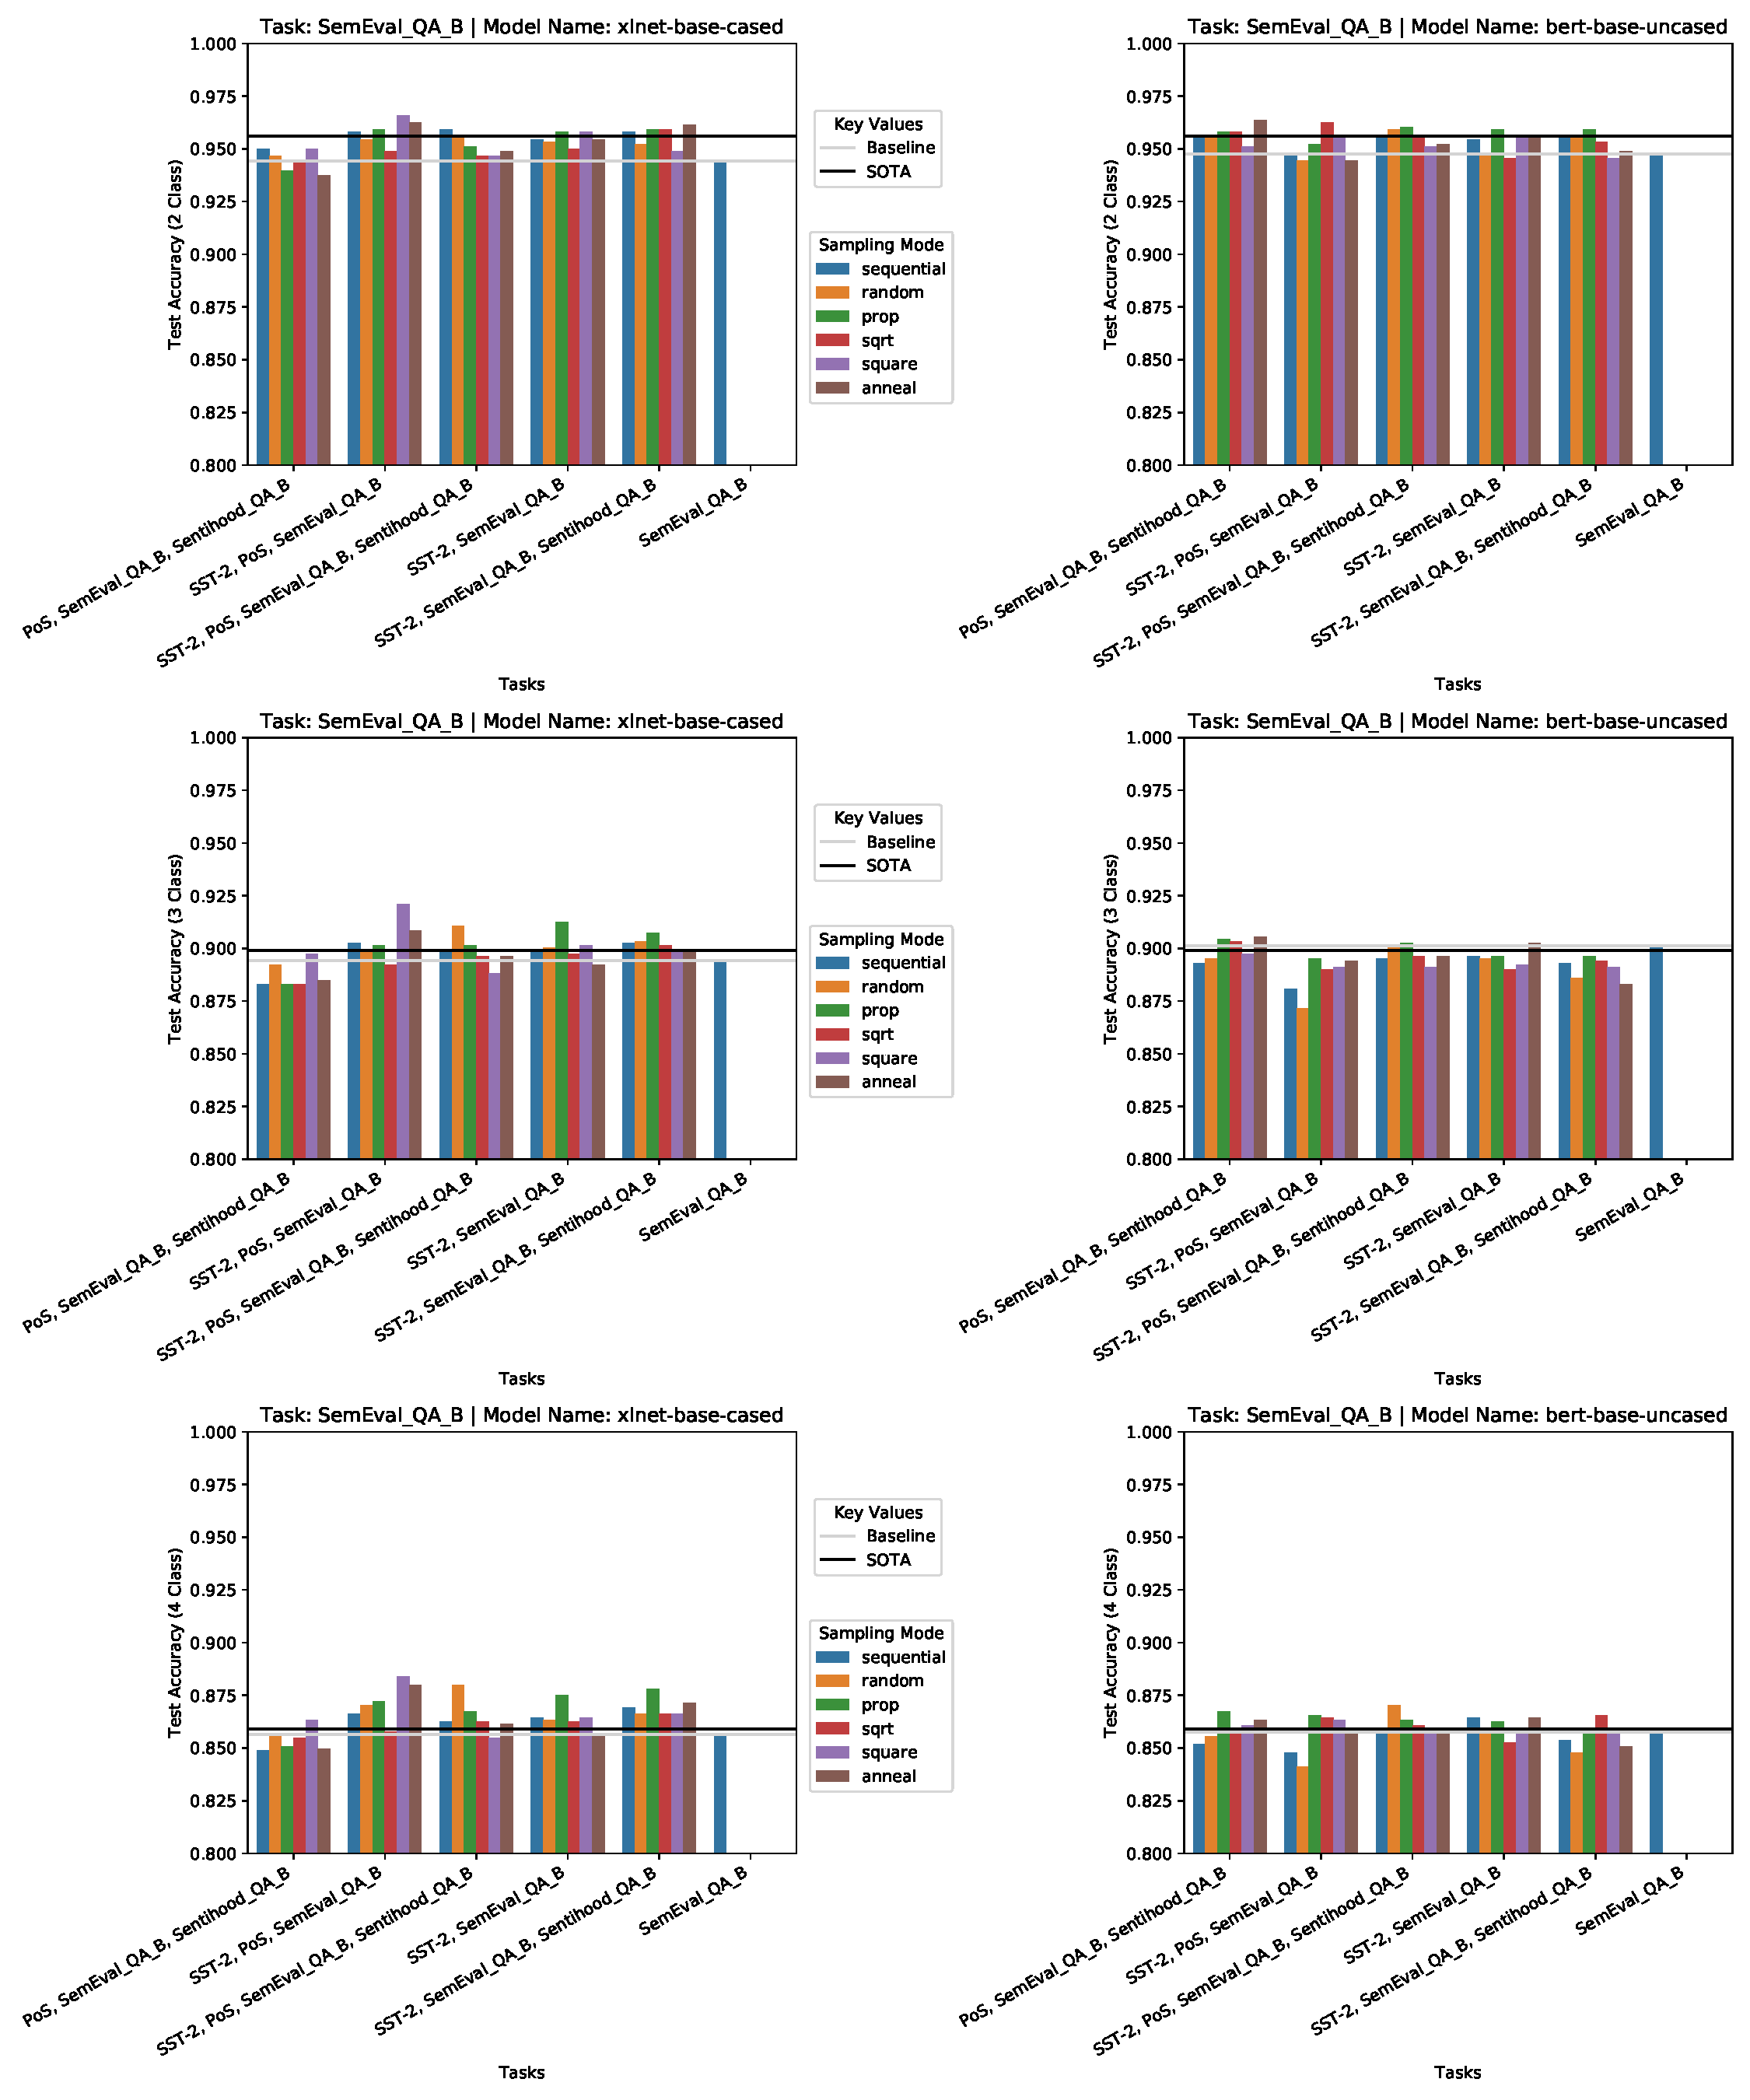
\includegraphics[width=1.3\textwidth]{SemEvalResults.pdf}}%
	\captionof{figure}{SemEval \{2,3,4\}-way accuracies on BERT and XLNet for our sampling modes}
	\label{fig:experiments:semevalaccs}
\end{figure}

\begin{figure}
	\makebox[\textwidth][c]{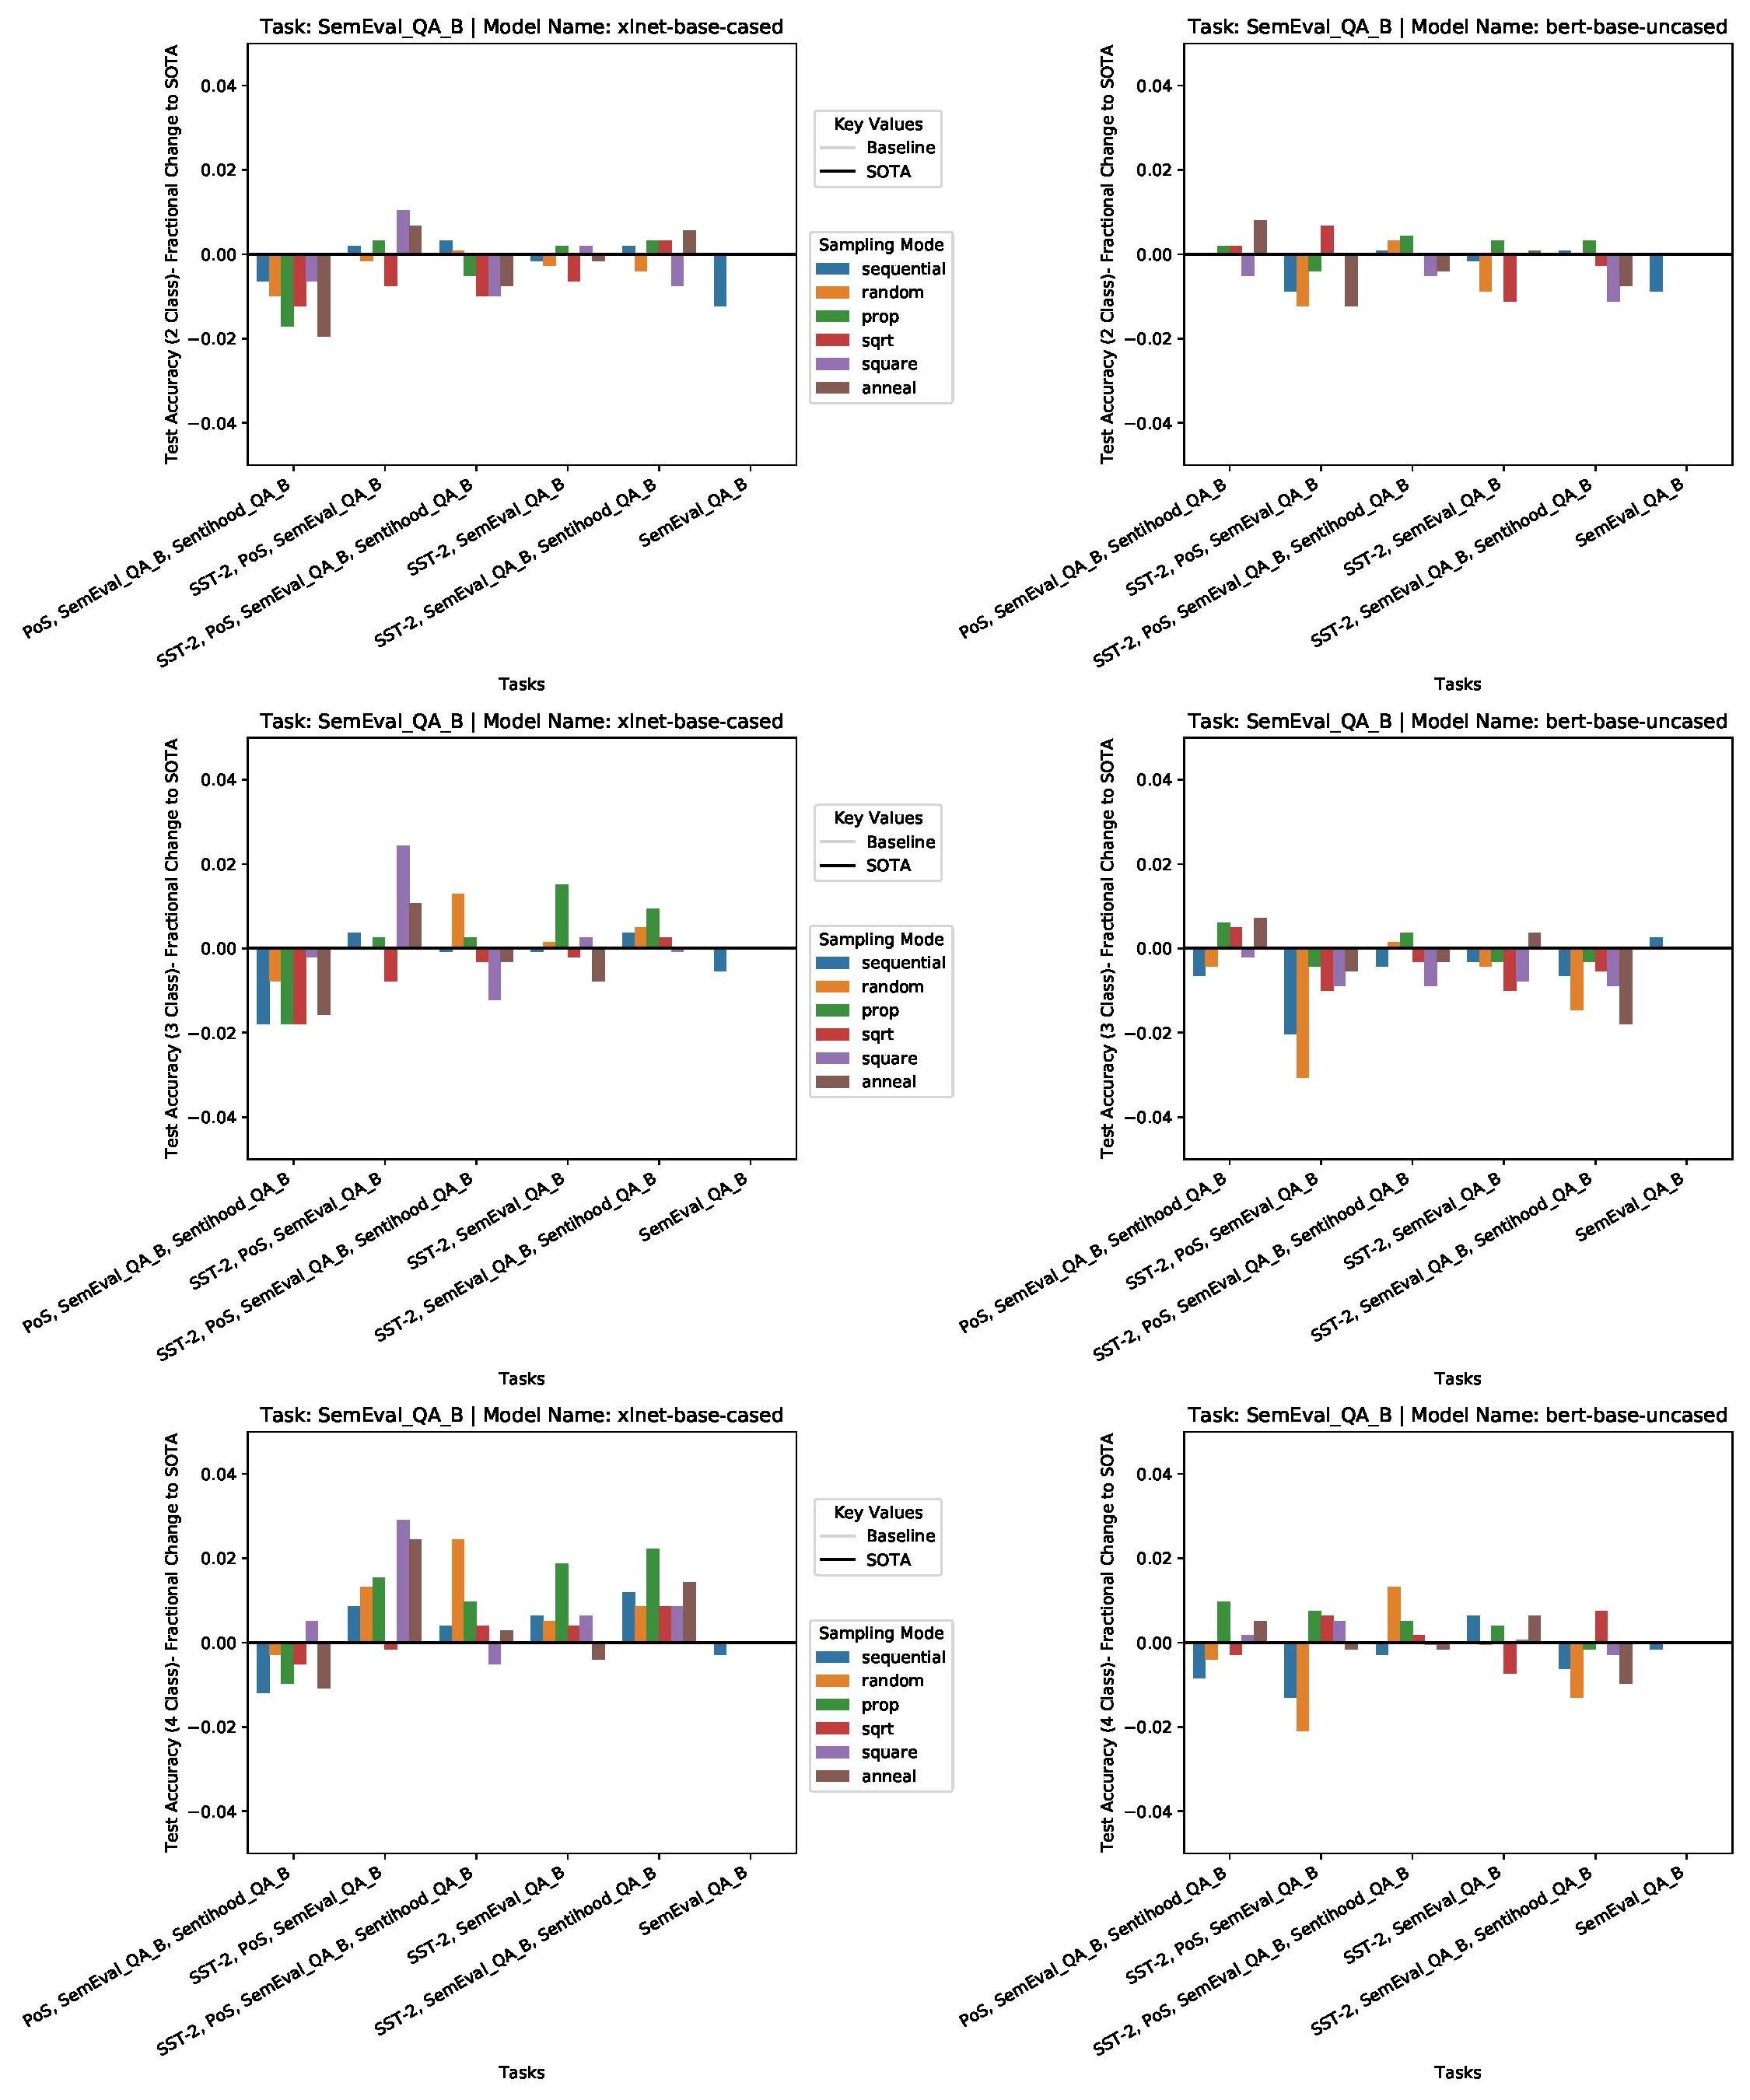
\includegraphics[width=1.3\textwidth]{SemEvalResults_relative.pdf}}%
	\captionof{figure}{SemEval \{2,3,4\}-way accuracies relative to SOTA performance on BERT and XLNet for our sampling modes}
	\label{fig:experiments:semevalaccsrelative}
\end{figure}

\begin{figure}
	\makebox[\textwidth][c]{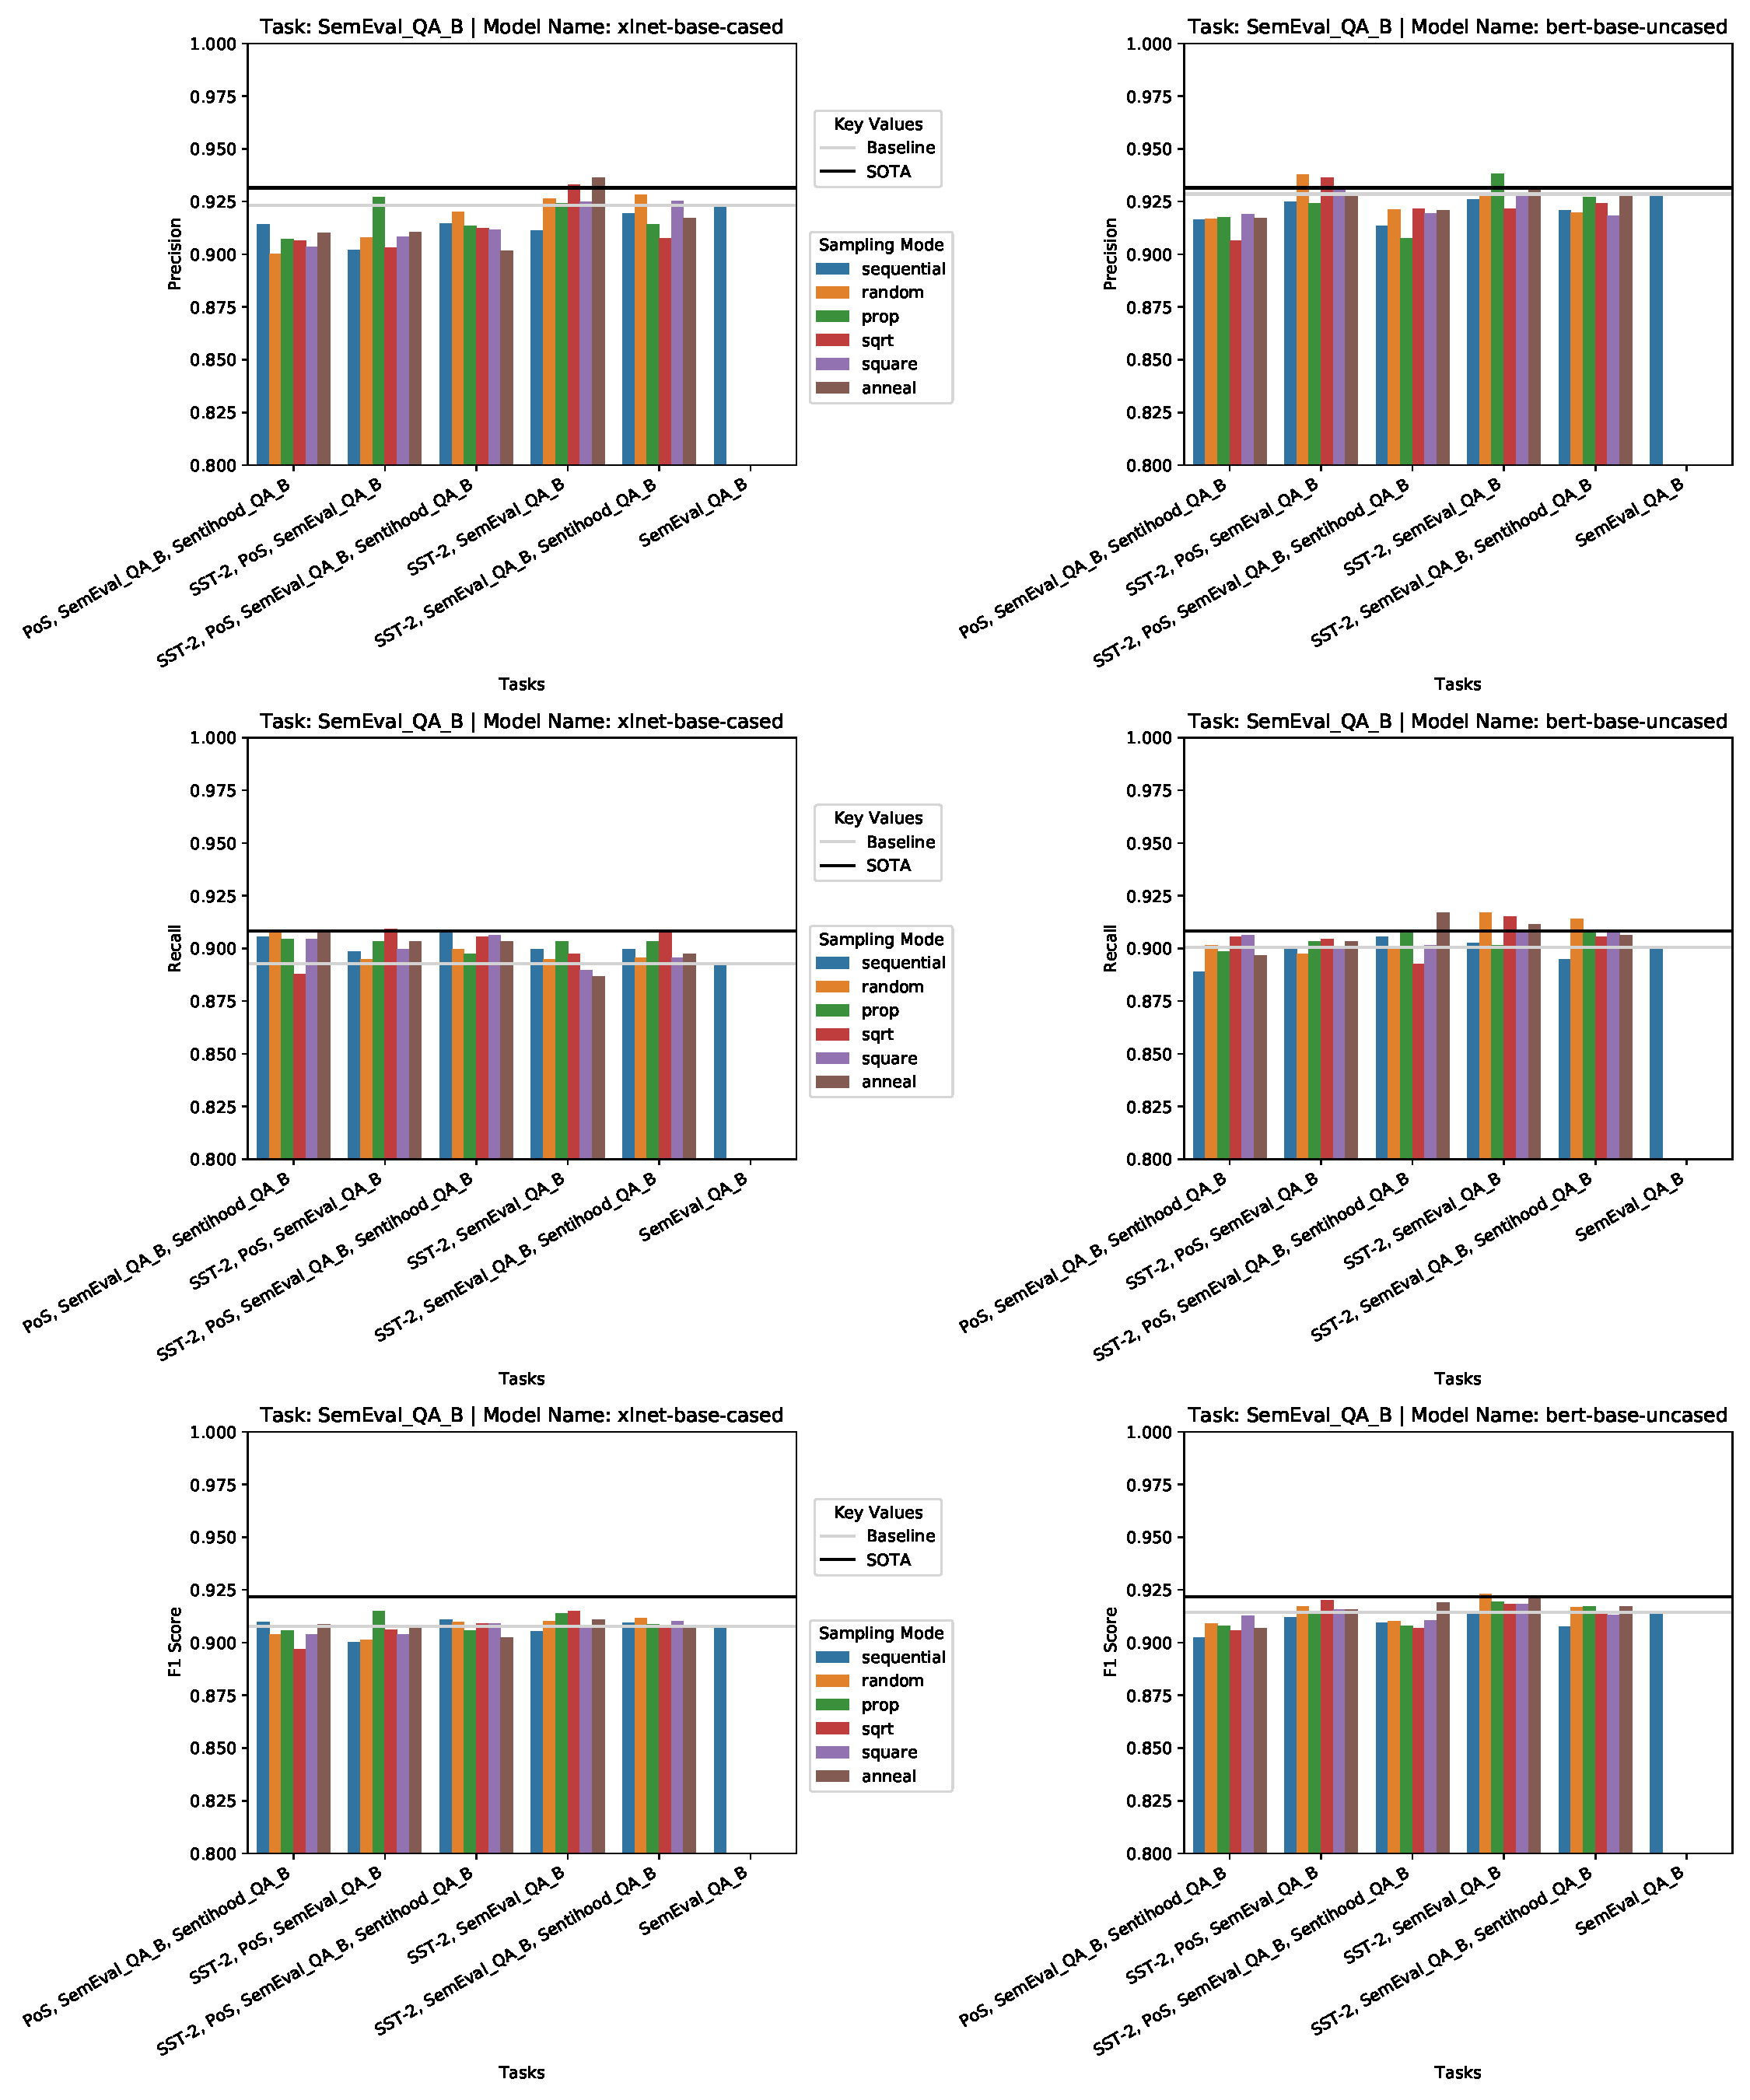
\includegraphics[width=1.3\textwidth]{SemEvalResultsPRF.pdf}}%
	\captionof{figure}{SemEval Precision, Recall and $F_1$ Scores on BERT and XLNet for our sampling modes}
	\label{fig:experiments:semevalprf}
\end{figure}

\subsection{NLI Pretraining Task Importance} \label{section:experiments:nlipretrainingimportance}
As mentioned in Sections \ref{section:background:bert} and \ref{section:background:xlnet}, there are key differences in the pretraining procedure of each of our two language models under consideration: the next sentence prediction task. BERT was trained with this binary next sentence prediction task whereas XLNet was not. As discussed in Section \ref{section:background:tabsasentenceconstruction}, the performance for BERT on this ABSA task using this auxilliary sentence construction method was put down to its ability to leverage knowledge from its pretraining task enabling it to better fine tune at binary QA and NLI tasks.
We empirically validate this conjecture through extensive testing that was omitted from the original paper. Indeed, we show this in the results in Figure \ref{fig:experiments:semevalaccs}. We see that the baseline task performance (i.e just pretraining on SemEval\_QA\_B) on XLNet was \textit{worse} than BERT on the ABSA task using this method, despite it being a better language model than BERT on 20 ``classic" downstream tasks \cite{Yang2019}. This suggests that, since the (T)ABSA tasks are more difficult than the NLI/QA tasks in GLUE, it is important to have this NLI pretraining procedure for more difficult downstream tasks. This validates the importance of the NLI pretraining task, and was an important subpart of this investigation. We see, in spite of this, that the XLNet models are able to overcome the SOTA barriers using multitask learning with our task hierarchy.
We discuss later, in Section \ref{section:extensions:subtasks}, about how we might have been able to improve performance by additionally incorporating a NLI/QA task at test time, but this was omitted from this investigation. 

While it is true that XLNet is able to recover performance with downstream multitask learning, the benefits of incorporating a QA/NLI task are clear since BERT achieves a better initial performance, making a case for its inclusion as a pretraining task, and thus we conclude that the NLI task must have a role to play in order to better generalise to this complicated ABSA QA\_B type setup, as defined in Section \ref{section:background:tabsasentenceconstruction}. This aligns with the original papers of BERT and ERNIE 2.0 \cite{Devlin2018, Sun2019a}, but contrary to XLNet and RoBERTa \cite{Yang2019, Liu2019} (although we are using a different, more complicated downstream task than those tested in the papers). This means we can expand and give additional evidence that pretraining with additional tasks does help a models transfer learning abilities in the single task setting.

\subsection{Analysis of Results}
As mentioned in Section \ref{section:experiments:nlipretrainingimportance}, we established that the baseline performance of XLNet is worse than that of BERT, which is interesting in its own right. We see that, when utilising multitask learning, we outperform state of the art according to every accuracy metric as displayed in the tables in Section \ref{section:experiments:allsotaresults}. More importantly in terms of experimental validation of our methodology, we see from Table \ref{table:experiments:semevalresults} that all the models that beat SOTA 2 way accuracy sample according to our preimposed task hierarchy, commonly sampling proportionally rather than sequential or randomly which were our baselines. Unsurprisingly, the top results utilise the multitask representations of the sentiment task as well as the PoS task with the best performing model using the squared sampling schema. This extremises the importance of SemEval\_QA\_B over the other tasks whilst leveraging representations learned from subtasks of PoS and SST-2 as expected (which makes sense intuitively since both sentiment and PoS labelling tasks are useful in ABSA). This validates the approach and motivation we proposed in Section \ref{section:methodology:taskstructure}.

We additionally find that each of the top 5 performing models for binary classification for each of the model classes use the sampling schemas we defined in this thesis as opposed to just sequential sampling, thereby validating the importance of defining these schemas. We report relative improvements in an already high SOTA accuracy score of greater than 1\% in the best case. This can be seen in Table \ref{table:experiments:semevalresults}.

Where this multitask learning seems to improve results is in the much harsher metrics. We find that an \texttt{xlnet-base-cased} model fine tuning with tasks \{SST-2, PoS, SemEval\_QA\_B\} using the square sampling schema achieves a 4 way accuracy of 0.8839, which is a 0.02 absolute improvement on this metric and an impressive 2.9\% relative increase on SOTA. It seems that these alternative representations enable the model to better classify classes with fewer labels in the dataset (since there is a severe label imbalance for the ``neutral" and ``conflict" classes), probably since the model does not overfit and learn to optimise just the two label setting, but instead favouring hypotheses that generalise well amongst all tasks (relating back to our discussion in Section \ref{section:background:multitask}, where the tasks act as regularisers for the model).

We see that, from Figure \ref{fig:experiments:semevalprf}, when considering Precision, Recall and F1 Scores, in general we see that \texttt{bert-base-uncased} actually performs better than XLNet in terms of beating the SOTA scores. We also conjecture this is due to the importance of the NLI pretraining task.

\begin{center}
	\resizebox{\textwidth}{!}{%
		\begin{tabular}{lllrll}
			\toprule
			Model Name &                                     Tasks & Sampling Mode &  Test Acc. (2 Class) & Absolute Increase to SOTA & Relative Increase to SOTA \\
			\midrule
			\multirow{5}{*}{bert-base-uncased} &         PoS, SemEval\_QA\_B, Sentihood\_QA\_B &        anneal &                        0.963595 &                      0.01 &                     0.79\% \\
			&                  SST-2, PoS, SemEval\_QA\_B &          sqrt &                        0.962457 &                      0.01 &                     0.68\% \\
			&  SST-2, PoS, SemEval\_QA\_B, Sentihood\_QA\_B &          prop &                        0.960182 &                       0.0 &                     0.44\% \\
			&                       SST-2, SemEval\_QA\_B &          prop &                        0.959044 &                       0.0 &                     0.32\% \\
			&       SST-2, SemEval\_QA\_B, Sentihood\_QA\_B &          prop &                        0.959044 &                       0.0 &                     0.32\% \\
			\hline
			\multirow{5}{*}{xlnet-base-cased}  &                  SST-2, PoS, SemEval\_QA\_B &        square &                        0.965870 &                      0.01 &                     1.03\% \\
			&                  SST-2, PoS, SemEval\_QA\_B &        anneal &                        0.962457 &                      0.01 &                     0.68\% \\
			&       SST-2, SemEval\_QA\_B, Sentihood\_QA\_B &        anneal &                        0.961320 &                      0.01 &                     0.56\% \\
			&                  SST-2, PoS, SemEval\_QA\_B &          prop &                        0.959044 &                       0.0 &                     0.32\% \\
			&       SST-2, SemEval\_QA\_B, Sentihood\_QA\_B &          prop &                        0.959044 &                       0.0 &                     0.32\% \\
			\bottomrule
	\end{tabular}}
	\captionof{table}{SemEval\_QA\_B 2 way (binary) accuracy results (restricted to the top 5 of each model that beat SOTA performance)}
	\label{table:experiments:semevalresults}
\end{center}


\section{An Overview of SOTA Results Achieved}
\label{section:experiments:allsotaresults}
\begin{center}
	\resizebox{\textwidth}{!}{
	\begin{tabular}{c@{\qquad}cccc@{\qquad}}
		\toprule
		\multirow{2}{*}{\raisebox{-\heavyrulewidth}{Metric}} & \multicolumn{4}{c}{SemEval\_QA\_B}\\
		\cmidrule{2-5}
		& Previous SOTA & Our SOTA & Model Name & Tasks (Sampling Mode) \\
		\midrule
		F1\_Score                         &        0.9218 &              0.922926 &       BERT & SST-2, SemEval\_QA\_B (random) \\
		Precision                        &        0.9315 &              0.938071 &         BERT & SST-2, SemEval\_QA\_B (prop) \\
		Recall                           &        0.9083 &              0.917073 &       BERT & SST-2, SemEval\_QA\_B (random) \\
		2 Class Accuracy  &        0.9560 &               0.96587 &  XLNet & SST-2, PoS, SemEval\_QA\_B (square) \\
		3 Class Accuracy   &        0.8990 &              0.920863 &  XLNet & SST-2, PoS, SemEval\_QA\_B (square) \\
		4 Class Accuracy   &        0.8590 &              0.883902 &  XLNet & SST-2, PoS, SemEval\_QA\_B (square) \\
		\bottomrule
	\end{tabular}}
	\resizebox{\textwidth}{!}{
		\begin{tabular}{c@{\qquad}cccc@{\qquad}}
			\toprule
			\multirow{2}{*}{\raisebox{-\heavyrulewidth}{Metric}} & \multicolumn{4}{c}{Sentihood\_QA\_B}\\
			\cmidrule{2-5}
			& Previous SOTA & Our SOTA &Champion Model & Tasks (Sampling Mode) \\
			\midrule
			F1\_ Score & 0.879 &                0.928814 & XLNet &       SST-2, SemEval\_QA\_B, Sentihood\_QA\_B (prop) \\
			Aspect AUC           &           0.975 &                0.978023 &                      XLNet & SST-2, Sentihood\_QA\_B (sqrt) \\
			Sentiment AUC          &           0.970 &                0.973881 &  XLNet & SST-2, SemEval\_QA\_B, Sentihood\_QA\_B (sequential) \\
			Strict Aspect Accuracy  &           0.798 &                0.876201 &                      XLNet & SST-2, Sentihood\_QA\_B (prop) \\
			\bottomrule
	\end{tabular}}
	\captionof{table}{SOTA results for the TABSA tasks: SemEval and Sentihood}
	\label{table:experiments:sotaresults}
\end{center}

We see that on the TABSA and ABSA task, of which there are 10 key metrics, 7 out of 10 (70\%) of our champion models utilise our task hierarchy sampling schemas, with the most popular being square and proportional.

We see that, whilst improvements do come from the newer model (XLNet vs BERT), multitask learning further improves the previous SOTA scores, and sampling using our sampling schemas improves it even more. It is a combination of these three aspects that boosts our SOTA scores up to the levels reported in Table \ref{table:experiments:sotaresults}, particularly on Sentihood (TABSA). The graphs for the TABSA dataset are not discussed in this section, and the reader is referred to Appendix \ref{appendix:additionalfindings} for an overview of additional findings.

\section{Streetbees Results}
At an early stage in the process, we conducted this methodology using the Streetbees datasets. This was useful in testing the end to end scripts for running experiments across both models (BERT and XLNet) and a few sampling modes (we chose sequential, since it is the baseline, and prop, since it demonstrates our novel idea effectively). We did not use all sampling modes since the company was happy with a ``good" solution utilising this technology, and the models were only intended to provide as a proof-of-concept.

\subsection{Multilabel Emotion Results}
The main company dataset we will be considering is the question \textit{``How do you feel?"}, to which there is a fixed emotion set of 34 nontrivial\footnote{a label is defined as nontrivial if there was at least 100 instances of it in the entire dataset of c. 50k datapoints} labels. This data is multilabelled, thus requiring a sigmoid for each label. We thus choose to use the ABSA QA\_\textbf{B} type setup, since we get a probability of each emotion class by default since that is how the data is set up as well as the fact that these auxilliary supplementary questions mimic the way the question was asked to the users originally. The question that is augmented to the responses are \textit{``Do you feel $e$?"} for each emotion $e \in \mathcal{E}$, the set of all emotion classes.
\begin{center}
	\resizebox{\textwidth}{!}{%
		\begin{tabular}{lllrlll}
			\toprule
			& Model Name &   Tasks & Sampling Mode &  Precision & Recall & $F_1$ Score \\
			\midrule
			\multirow{2}{*}{Best Performing ($F_1$ Score)} &         \texttt{bert-base-uncased} &	SST-2, PoS, SemEval\_QA\_B, Streetbees\_Mood	& prop	& 0.910938	& 0.917683	& 0.914298 \\
			&  \texttt{xlnet-base-cased}	& SST-2, Streetbees\_Mood	& prop	& 0.900042	& 0.923563	& 0.911651 \\
			\hline
			\multirow{2}{*}{Baseline (Fine tuning, single task)}  & \texttt{bert-base-uncased}	& Streetbees\_Mood	& sequential	& 0.901068	& 0.918336	& 0.909620 \\
			& \texttt{xlnet-base-cased} &	Streetbees\_Mood	& sequential	& 0.895202	& 0.926394	& 0.910531 \\
			\bottomrule
	\end{tabular}}
	\captionof{table}{Streetbees Results, showing the best performing model by $F_1$ Score compared to the baseline fine tuning models}
	\label{table:experiments:streetbeesresults}
\end{center}

The key metric that we focus on is maximising the $F_1$ Score, which is the harmonic mean of precision and recall. What we see in the results is that the best performing model for both BERT and XLNet utilise the proportional sampling scheme as opposed to ``regular" sequential multitask learning, further validating the utility of these sampling schemas. However, the baseline models still perform admirably, with the XLNet model baseline performing very similarly to the best performing one, and the BERT baseline only achieving an $F_1$ score of 0.05 less.

While the results are important, what is more useful is the impact the model has had on the business. In a presentation to the CEO, we stress tested the model. It was obviously able to match key words corresponding to the emotion categories, but more importantly it was able to do powerful inferencing steps. One standout example was the phrase \textit{``I miss my brother"}, from which the model was able to infer both sadness and loneliness categorisations; demonstrating the power of these contextualised models. Importantly from a business perspective, the marginal gains achieved by this multitask setup might be considered negligible and there is a tradeoff between good metric scores and the additional training time required for the joint multitask models to train.

The model was then additionally applied to a foodstuff ontology. A similar setup was utilised: this time the users were asked \textit{``What are you eating?"} and certain categories were identified as a labelling/coding schema such as \textit{``Chicken"} and \textit{``Wrap"} with multiple labels possible if the person was eating e.g a chicken wrap, and the responses to the questions were fed into the language models with the augmented question: \textit{``Are you eating $f$?"} for each $f$ in the food categories. This model enjoyed similar successes to the previous example, but investigations as to its efficacy are still ongoing as the company intends to incorporate image data to form a multimodal model since the text data is much noisier in this instance. This multitask multimodal system is currently being developed by researchers at the company; a component of which is the language models we have implemented for the text classification. All of the multitask language modelling frameworks have been implemented into the companies internal codebase and code reviewed.

\subsection{Generalisation Capabilities}
An interesting development from the internal conversations at the company would be how these models would generalise to a new aspect, or emotion in this case. Since the auxilliary question setup is emotion agnostic, we simply added a new emotion category to the labels: ``pride" and fed in input sentences to the model. We found that the model was only really able to ascertain exact key word matches, since it still had a learned embedding of ``pride" and was in some sense doing a similarity between the input sentence and this emotion word embedding, but it was unable to capture more nuance such as \textit{``My son just won an award"} where more inference would be required and the model has not been fine tuned to do this.

It is relatively easy for the business to label a few examples of datapoints following a new class label, such as pride, but it is unclear if the model would be able to classify them effectively in this multitask setup, since generally thousands of examples are needed (as the model performed best in practice on more common labels, as is expected). We thus turned our attention to meta learning, and explored its utility in this text classification generalisation space. We return to this idea in Section \ref{section:extensions:meta}.

\section{Preliminary Experiments}
\subsection{Ensuring Baseline Performance}
Since our architecture was much more general than typical fine tuning, and was coded from scratch but building upon a lot of various libraries, we had to ensure that in the case of a single task we recreated the performances quoted in our key literature papers. This was the first challenge. We also introduced a more stable and generalisable data ingestion format, that abstracts away a lot of the hard coded implentations for various datasets. We wrote scripts that converted each of our datasets into this standardised format and release these reformatted dataset (split) publicly.

 In particular, we focused first on recreating the SST-2 performances reported in the official BERT and XLNet papers \cite{Devlin2018, Yang2019}, since these papers were well written, with a full overview of hyperparameter choices and results, as well as the fact that the data was taken from a source that is well maintained (i.e not outdated mirror links) and is often cited. Once we recreated the performance for this, we moved on to recreating the performance quoted in the TABSA Auxilliary Sentence paper \cite{Sun2019}.

This proved more challenging, since their code was uncommented and not written for our use case. Thus, it required a lot of code rewriting and refactoring, in particular of the evaluation logic and the data formulation scripts, in order to reimplement the functionality for our purposes, as well as extending it to the more general setting we were considering. Additionally, we commented the code and abstracted various sections for open sourcing and reusability by the research community. The hyperparameters were loosely covered, and the assumption was made that all those hyperparameter settings not reported were left as the defaults in the BERT paper. With these assumptions, we were able to emulate the base performance of that in the paper.

\subsection{Gradual Unfreezing of Base Language Model Layers} \label{section:experiments:unfreezing}
As mentioned in Section \ref{section:methodology:modelsetup}, the library has support for the gradual unfreezing of the base layers. This was going to be one aspect of the multitask schema that was going to be investigated, with the hypothesis that the instantiation of the base weights provides a good initial starting point, and if we froze all layers except the final embedding layer, but as training progressed started to unfreeze deeper layers through time, we would be able to fine tune our embeddings better. We found that this was unhelpful in practice and the results were not much different from just instantiating the base model and letting gradients backpropagate through the entire model, so was omitted after this early testing stage as to not cloud the results with an unnecessary layer of complexity.

\subsection{Multitask learning for Sentiment Classification} \label{section:experiments:sentimentonly}
We began by looking at multitask learning for Sentiment Classification. In particular, we took the two most popular sentiment classification datasets: SST-2 and IMDB and tried initial experiments that would:
\begin{enumerate}[a.]
	\item Test the end to end architecture of our model on multiple tasks, and ensure the reporting was correct, as described in Section \ref{section:methodology:reporting}.
	\item Ascertain whether different tasks contributed to better learned representations and word embeddings for each seperate sentiment downstream task individually.
\end{enumerate}

These initial experiments combined the remarks in Section \ref{section:experiments:taskdistributions} with the task priorities as defined in Table \ref{table:methodology:datasets}. The results are shown in Figure \ref{fig:experiments:sentimentmultitaskresults}.

From this, we see that multitask learning does marginally improve performance on the both tasks when we use the \texttt{bert-base-uncased} model but does not yield any improvements when using the \texttt{xlnet-base-cased} model. This could be because the pretraining of XLNet was more effective at capturing word embeddings that are useful for sentiment tasks, and learning different representations in this instance does not yield any improvements. We concluded that it would not be efficient to include both tasks in our general (T)ABSA multitask learning setup and both performed similarly and, as we discuss in Section \ref{section:experiments:taskdistributions}, the number of experiments we run scaled exponentially with the number of tasks. The improvements from learning varied sentiment based word embeddings only enables the successful classification of a handful of additional examples, and thus, since two sentiment tasks seemed redundant, we decided to continue with \textit{only} the SST-2 task as a supporting sentiment task since it was the most common dataset on which sentiment analysis models are benchmarked.

\begin{center}
	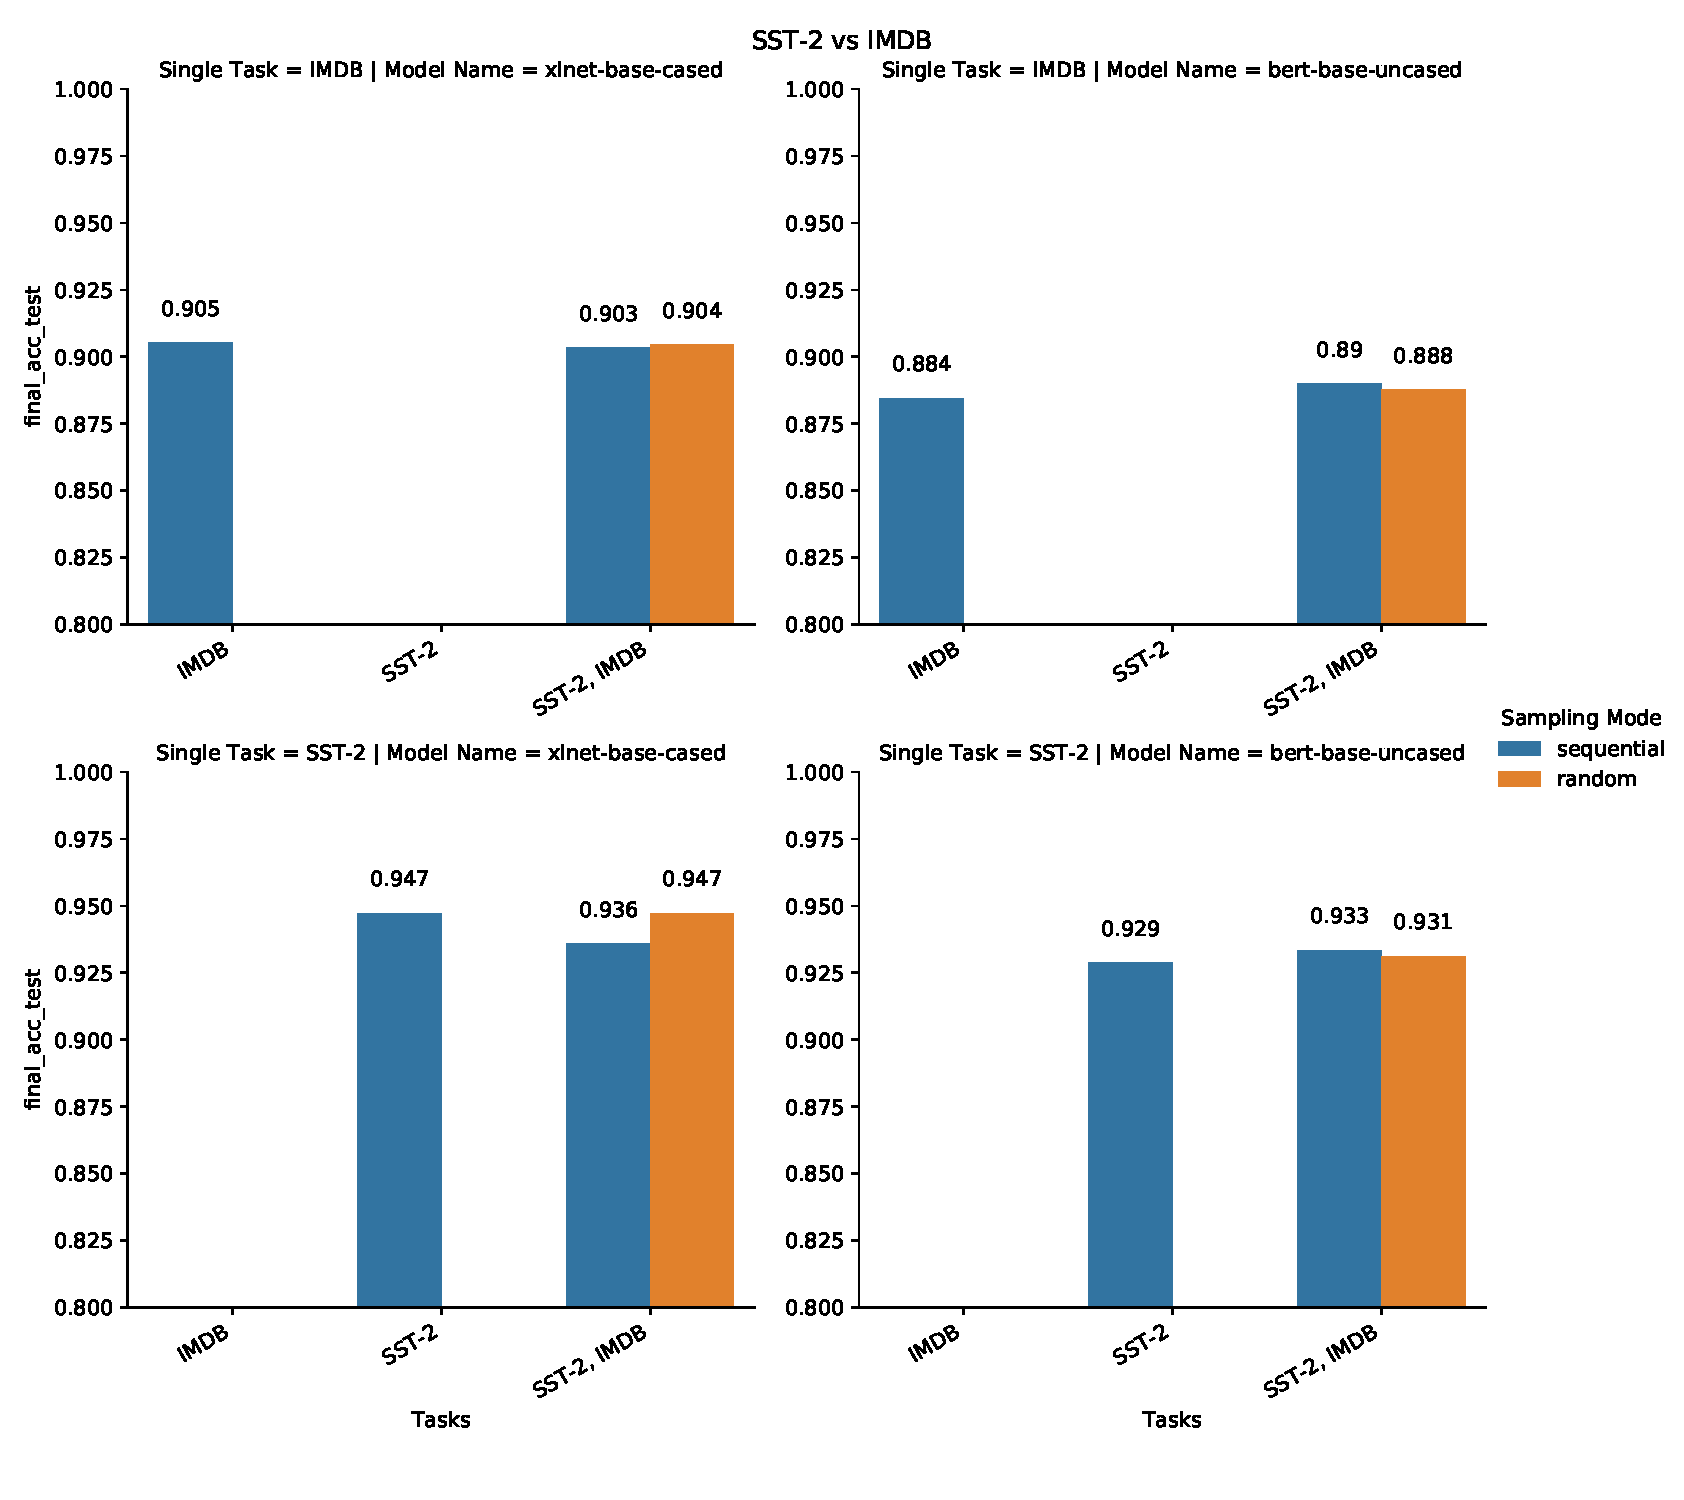
\includegraphics[width=.8\textwidth]{SST2vsIMDB.pdf}
	\captionof{figure}{SST-2 vs IMDB in the single task and multitask learning setting}
	\label{fig:experiments:sentimentmultitaskresults}
\end{center}

\section{Success of the Sampling Schemas}
The previous section highlights the results of the models, showcasing the importance of a sampling schema to best leverage information from related subtasks when attempting to solve a difficult NLP task. We see that, in general, the best performing models do in fact utilise our novel sampling schema in some way, performing better than baseline multitask learning training i.e sequential (or ``round robin") task sampling. 

Unfortunately, there is no ``stand out" sampling schema. In terms of granular accuracies, the square sampling mode clearly wins on the ABSA task, and in general any type of proportional sampling gets SOTA results. The task weightings were arbritrarily defined just to showcase the idea effectively, and so a clear extension is to beter define these task weights. This is one such extension that we discuss in Section \ref{section:extensions:taskweightings}.

In general, looking at the Figures \ref{fig:experiments:semevalaccs} - \ref{fig:experiments:semevalprf} the sampling schema that often outperforms SOTA is actually the annealing strategy. This strategy is interesting, since it samples proportional to our task hierarchy initially in order to quickly learn good representations, but as the number of training steps increases the sampling schema becomes more uniform over $\mathcal{T}$; a type of smoothing process. This was motivated by the fact that early in the fine tuning process we want to take gradient descent steps using the batches of our main task and update the weights to good local minima to solve the task, but as time goes on and a good local minima is found, we want to use representations from all tasks to further refine our weights. It seems this strategy works best overall, and investigations that vary the annealing constant might prove a useful extension.

\section{Remark on Task Distributions for Experimental Optimisation} \label{section:experiments:taskdistributions}
Although it may look like when we want to run a set of experiments on tasks $\mathcal{T}$ there are:
\begin{align*}
\underbrace{2}_{\text{\#Models}} \cdot \underbrace{6}_{\#Schemas} \cdot \underbrace{\sum \limits_{r=1}^{|\mathcal{T}|} {|\mathcal{T}| \choose r}}_{=2^{|\mathcal{T}|} - 1 \text{ i.e. \# of tasks of length } r= 1,2,\dots, |\mathcal{T}|}
\end{align*}
such experiments, which scales exponentially badly, there are a few (obvious) tricks we can utilise to reduce the number of experiments, which we break down as a series of observations:
\subsubsection{Observation 1: The Single Task Setting}
In this setting, all sampling modes are equal, irrespective of the task priority. So, in this setting, we just consider the sequential schema, but really this is just normal fine tuning.

\subsubsection{Observation 2: The Two Task Setting}
\begin{prop}
	In this setting, if we have two tasks, say $\tau_i$ and $\tau_j$ of the same task priority, so that $w_{\tau_i} = w_{\tau_j}$, then the task distribution collapses onto two unique settings: the sequential (deterministic) setting, and the random setting.
\end{prop}
\begin{proof}
	For any $\alpha \in \mathbb{R}$, we have that if $w_{\tau_i} = w_{\tau_j} = w \neq 0$, say, then it follows that:
	\begin{align*}
	p_{\tau_i} = \frac{w_{\tau_i}^{\alpha}}{w_{\tau_i}^{\alpha} + w_{\tau_j}^{\alpha}} = \frac{w^{\alpha}}{w_{\tau_i}^{\alpha} + w_{\tau_j}^{\alpha}} = \frac{w_{\tau_j}^{\alpha}}{w_{\tau_i}^{\alpha} + w_{\tau_j}^{\alpha}} = p_{\tau_j}
	\end{align*}
	and so $p_{\tau_i} = p_{\tau_j} = p$ moreover that (since probabilities sum to 1), $p=\frac{1}{2}$. This can also be explicitly calculated since $p = \frac{w^{\alpha}}{w^{\alpha} + w^{\alpha}} = \frac{w^\alpha}{2w^\alpha}= \frac{1}{2}$ since $w \neq 0$.
	
	Since the sequential schema is nonrandom, it is different from the random schema, so must also be included.
\end{proof}

The proposition above enables us to eliminate the running of unneccessary experiments and sampling schemas, greatly reducing the computational time required.

\section{Training Choices} \label{section:experiments:training}
In this section, we detail the specific training choices that were made, including the hyperparameter setup and computing resources.
\subsection{Hyperparameters} \label{section:experiments:hyperparameters}
Unless otherwise stated, the experiments were all performed with hyperparameters as defaulted in the ABSA Paper \cite{Sun2019}, namely those outlined in Table \ref{table:experiments:hyperparameters}. Indeed, a thorough hyperparameter optimisation routine would have been far too computationally costly, even just over the most important hyperparameters like training batch size and learning rate. The point of this thesis was to investigate the multitask schema(s) alone, and thus fixing these hyperparameters offers a fair comparison between all schema choices. 

\begin{center}
	\begin{tabular}{||c | c||} 
		\hline
		Hyperparameter & Default Value  \\ [0.5ex] 
		\hline\hline
		Training Batch Size & 24 \\ 
		\hline
		Learning Rate & 2e-5  \\
		\hline
		Warmup Proportion & 0.1  \\
		\hline
		Number of Epochs & 4  \\
		\hline
		Annealing Constant & 0.9  \\
		\hline
		Random Seed & 42  \\
		\hline
	\end{tabular}
	\captionof{table}{The core hyperparameter default values we used throughout our testing}
	\label{table:experiments:hyperparameters}
\end{center}

Additionally, if correlates were found between optimal multitask schemas and performance improvements, hyperparameter tuning could be considered on a much smaller subset of experiments as an additional task. This is discussed in Section \ref{section:extensions:hyperparametertuning}.

\subsection{Computing Resources} \label{section:experiments:compute}
All the training was conducted on a single NVIDIA TITAN RTX GPU, named Stanley, which ran 24/7. Training of the experiments (iterating over model architecture choices as per Section \ref{section:experiments:languagemodels}, task distributions as per Section \ref{section:methodology:taskdistributions} and tasks as per Section \ref{section:methodology:datasets}) took circa 5 days, mostly owing to the large number of parameters present in the XLNet architecture.


